%% LyX 2.3.3 created this file.  For more info, see http://www.lyx.org/.
%% Do not edit unless you really know what you are doing.
\documentclass[12pt,english]{article}
\usepackage[T1]{fontenc}
\usepackage[latin9]{inputenc}
\usepackage{geometry}
\geometry{verbose,lmargin=1.5cm,rmargin=1.5cm}
\usepackage{float}
\usepackage{graphicx}

\makeatletter
\@ifundefined{date}{}{\date{}}
\makeatother

\usepackage{babel}
\begin{document}
\begin{figure}[H]
\centering{}%
\begin{minipage}[t]{0.45\columnwidth}%
\begin{center}
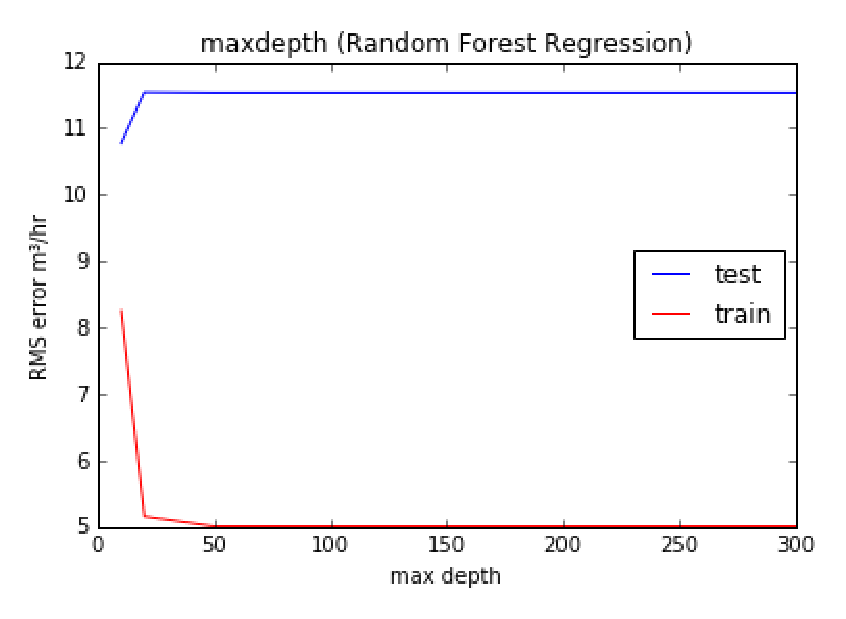
\includegraphics[width=6.5cm,height=6.5cm,keepaspectratio]{readings/rf/max_depth}\caption{Parameter tuned max depth}
\par\end{center}%
\end{minipage}\hfill{}%
\begin{minipage}[t]{0.45\columnwidth}%
\begin{center}
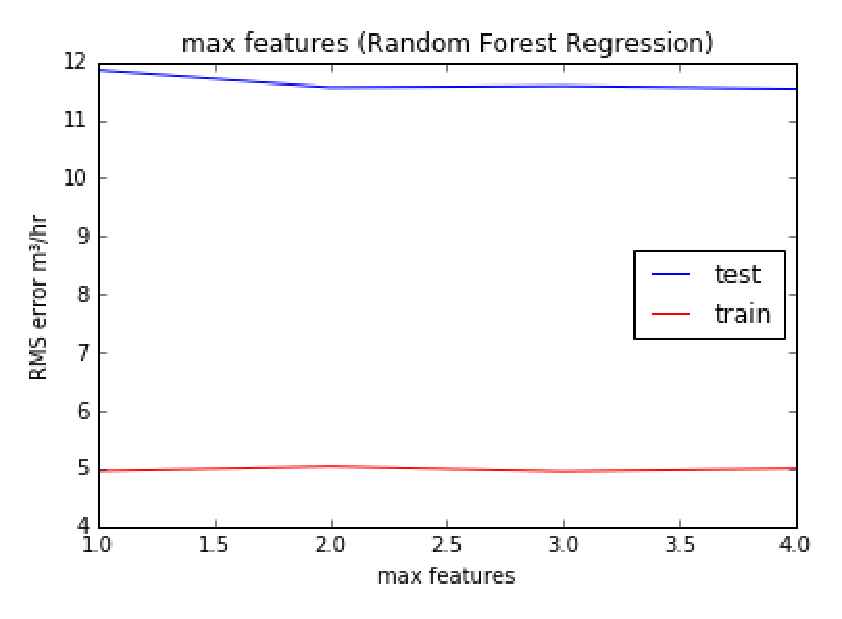
\includegraphics[width=6.5cm,height=6.5cm,keepaspectratio]{readings/rf/max_features}\caption{Parameter tuned max features}
\par\end{center}%
\end{minipage}
\end{figure}

\begin{figure}[H]
\centering{}%
\begin{minipage}[t]{0.45\columnwidth}%
\begin{center}
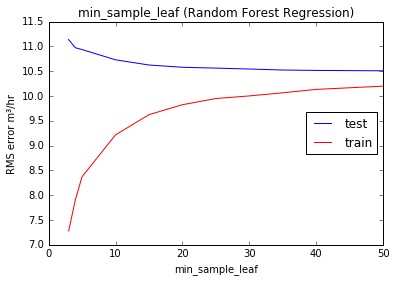
\includegraphics[width=6.5cm,height=6.5cm,keepaspectratio]{readings/rf/minsapmleaf}\caption{Parameter tuned min sample leaf}
\par\end{center}%
\end{minipage}\hfill{}%
\begin{minipage}[t]{0.45\columnwidth}%
\begin{center}
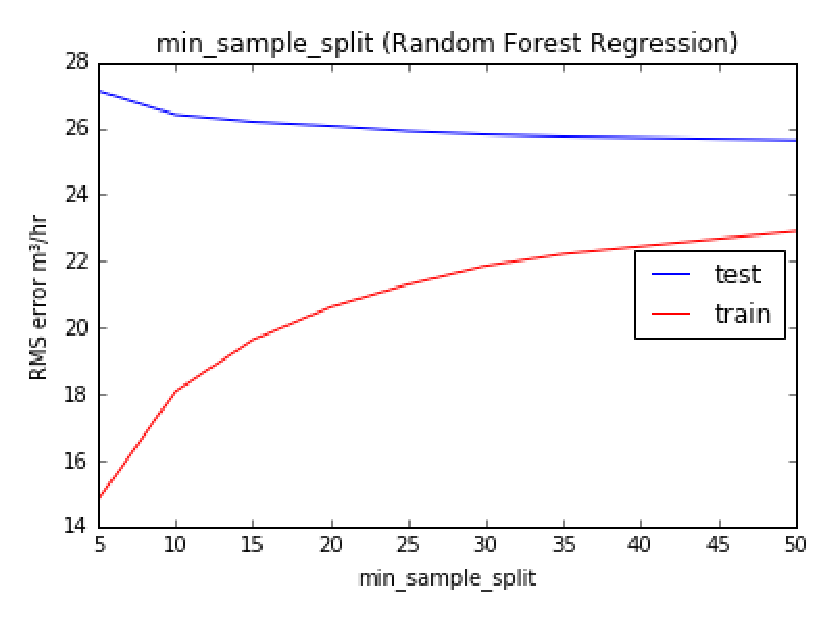
\includegraphics[width=6.5cm,height=6.5cm,keepaspectratio]{readings/rf/minsapmsplit}\caption{Parameter tuned min sample split}
\par\end{center}%
\end{minipage}
\end{figure}

\begin{figure}[H]
\begin{centering}
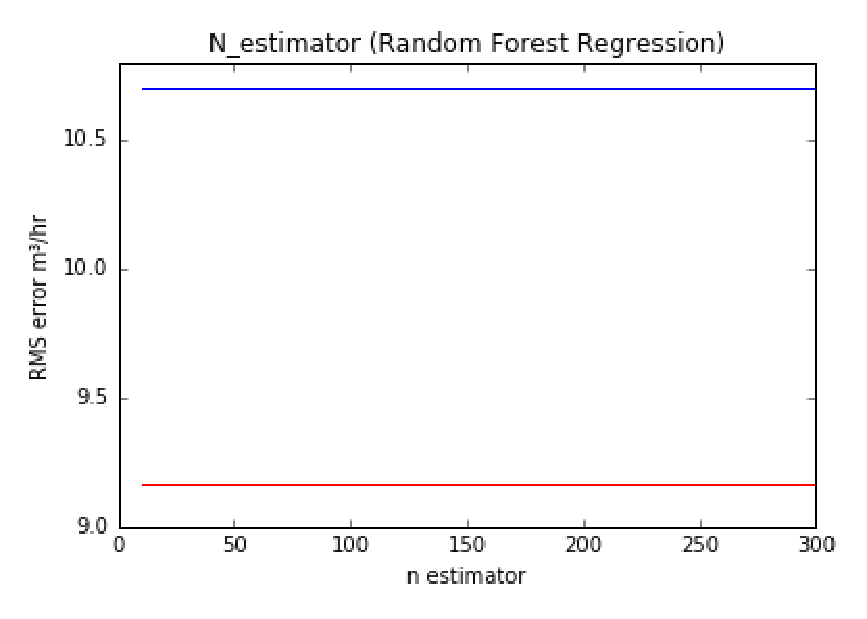
\includegraphics[width=6.5cm,height=6.5cm,keepaspectratio]{readings/rf/n_estimators}
\par\end{centering}
\caption{Parameter tuned n estimators}
\end{figure}
\begin{figure}[H]
\centering{}%
\begin{minipage}[t]{0.45\columnwidth}%
\begin{center}
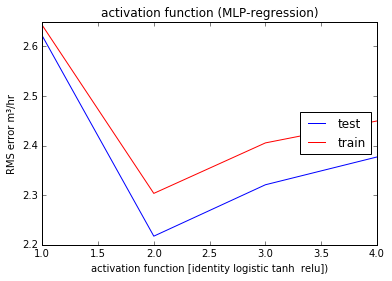
\includegraphics[width=6.5cm,height=6.5cm,keepaspectratio]{readings/mlp/actfunc}\caption{Parameter tuned activation function}
\par\end{center}%
\end{minipage}\hfill{}%
\begin{minipage}[t]{0.45\columnwidth}%
\begin{center}
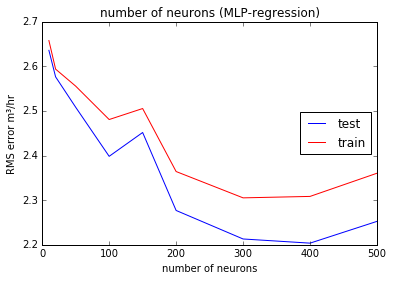
\includegraphics[width=6.5cm,height=6.5cm,keepaspectratio]{readings/mlp/noofnue}\caption{Parameter tuned number of neurons}
\par\end{center}%
\end{minipage}
\end{figure}

\begin{figure}[H]
\centering{}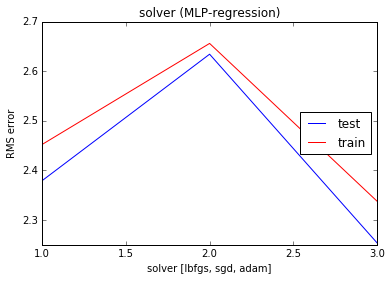
\includegraphics[width=6.5cm,height=6.5cm,keepaspectratio]{readings/mlp/solver}\caption{Parameter tuned solver}
\end{figure}

\begin{figure}[H]
\centering{}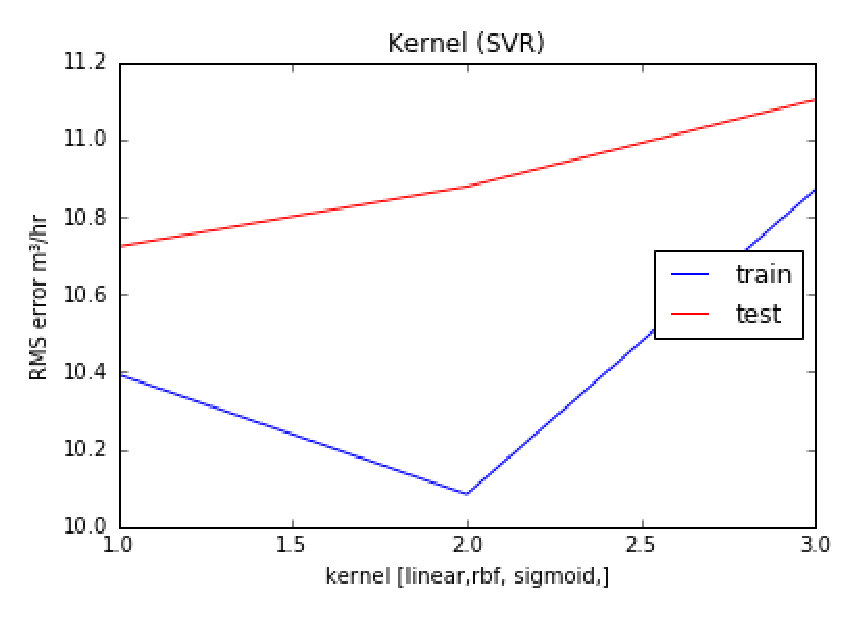
\includegraphics[width=6.5cm,height=6.5cm,keepaspectratio]{readings/svm/kernel}\caption{Parameter tuned kernel}
\end{figure}

\begin{figure}[H]
\centering{}%
\begin{minipage}[t]{0.45\columnwidth}%
\begin{center}
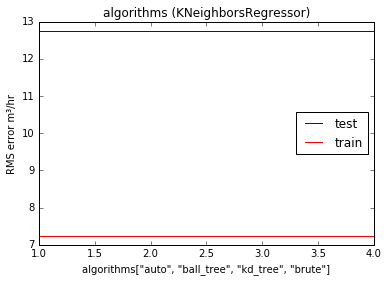
\includegraphics[width=6.5cm,height=6.5cm,keepaspectratio]{readings/knn/knn_algo}
\par\end{center}
\begin{center}
\caption{Parameter tuned algorithm}
\par\end{center}%
\end{minipage}\hfill{}%
\begin{minipage}[t]{0.45\columnwidth}%
\begin{center}
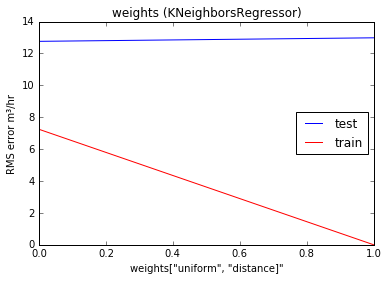
\includegraphics[width=6.5cm,height=6.5cm,keepaspectratio]{readings/knn/knn_weights}\caption{Parameter tuned weights}
\par\end{center}%
\end{minipage}
\end{figure}

\begin{figure}[H]
\centering{}%
\begin{minipage}[t]{0.45\columnwidth}%
\begin{center}
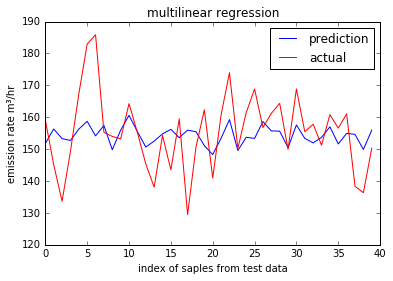
\includegraphics[width=6.5cm,height=6.5cm,keepaspectratio]{readings/mlr/mlp_testdata}\caption{Model tested on testing data}
\par\end{center}%
\end{minipage}\hfill{}%
\begin{minipage}[t]{0.45\columnwidth}%
\begin{center}
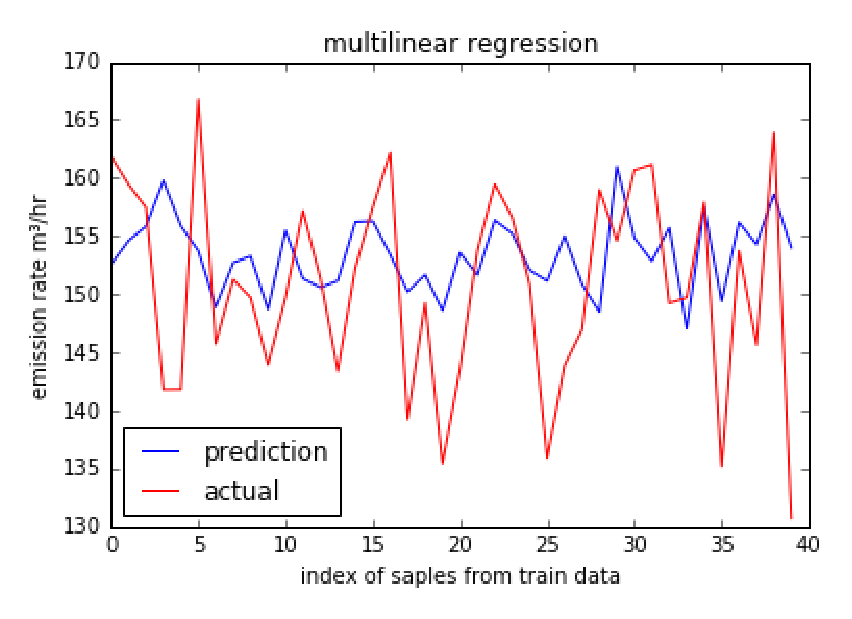
\includegraphics[width=7cm,height=7cm,keepaspectratio]{readings/mlr/mlp_traindata}\caption{Model tested on trainig data}
\par\end{center}%
\end{minipage}
\end{figure}

\begin{figure}[H]
\centering{}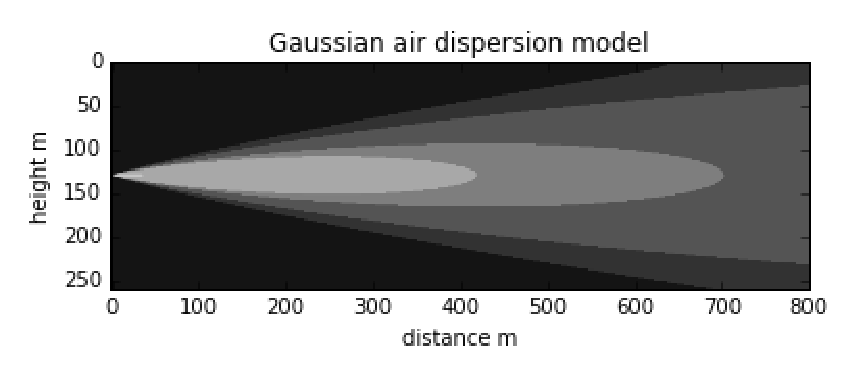
\includegraphics[width=9cm,height=9cm,keepaspectratio]{readings/gdm/result}\caption{Gaussian air dispersion model}
\end{figure}

\end{document}
